\documentclass{beamer}

\usepackage{graphicx}
\usepackage{multicol}
\usepackage[labelfont=footnotesize,textfont=scriptsize,bf]{caption}
\usepackage{subfig}
\usepackage{siunitx}
\usepackage{xcolor}
\usepackage{tikz}
\usetikzlibrary{shapes,arrows}
\usepackage{multicol}
\usepackage{ccicons}

\usepackage[utf8]{inputenc}
\usepackage[italian]{babel}
\usepackage[T1]{fontenc}

\graphicspath{{img/}}

\usetheme[hideothersubsections,width=60px]{PaloAlto}
\usecolortheme{wolverine}
\useinnertheme{rectangles}

\title[La piattaforma GIS \emph{Siponto Medievale}]{La piattaforma GIS \emph{Siponto Medievale}}
\subtitle{Laboratorio del corso di\linebreak\emph{Cultura materiale di età post classica}}
\author[Francesco de Virgilio]{Francesco de Virgilio \\ \texttt{\tiny francesco.devirgilio@openoia.org}}
\institute[O.I.A.~Open Idea for Archaeology]{
	%\inst{1}%
	OIA --- Open Idea for Archaeology%\\
	%\emph{Università degli Studi di Bari}
	}
	% \and
	% \inst{2}%
	% School for Computational Science\\
	% Florida State University}

\pgfdeclaremask{toplogo}{oia-logo}
\pgfdeclareimage[mask=toplogo,width=1.2cm]{oia-logo}{img/oia-logo}

\logo{\vbox{\vskip0.1cm\hbox{\pgfuseimage{oia-logo}}}}

\newcommand{\mysize}[1]{\footnotesize{\textbf{#1}}}

\begin{document}

\tikzstyle{block} = [rectangle, draw, fill=blue!20, text width=5em, text centered, rounded corners, minimum height=4em]
\tikzstyle{roundbox} = [rectangle, fill=white, draw=orange!80, very thick, double, text centered, rounded corners, minimum height=1em]
\tikzstyle{transitionbox} = [rectangle, fill=yellow, draw=orange!80, thick, text centered, rounded corners, minimum height=1em]

\AtBeginSection[]
	{
	\begin{frame}
		\frametitle{Sommario}
		\begin{multicols}{2}
			\tableofcontents[currentsection]
		\end{multicols}
	\end{frame}
	}

\begin{frame}
	\titlepage
\end{frame}

% -----------------------------------------------------

%\section*{Sommario}

	%\begin{frame}{Sommario}
		%\begin{multicols}{2}
			%\tableofcontents
		%\end{multicols}
	%\end{frame}
	
\begin{frame}{Istruzioni per l'uso}
    Queste slide sono strutturate per dare un'idea generale sulla gestione del dato archeologico nell'era del web 3.0. Non hanno la pretesa di essere esaustive. Alcuni argomenti sono stati estremamente semplificati per facilitarne la comprensione.\vfill
    Queste slide sono in licenza Creative Commons: puoi copiarle, condividerle con un amico!
    \begin{center}
        \Large{\ccbyncsa}
    \end{center}
\end{frame}

\part{Ora che si fa?}
	\frame{\partpage}

    \section{Vecchi e nuovi archivi}

        {
            \usebackgroundtemplate{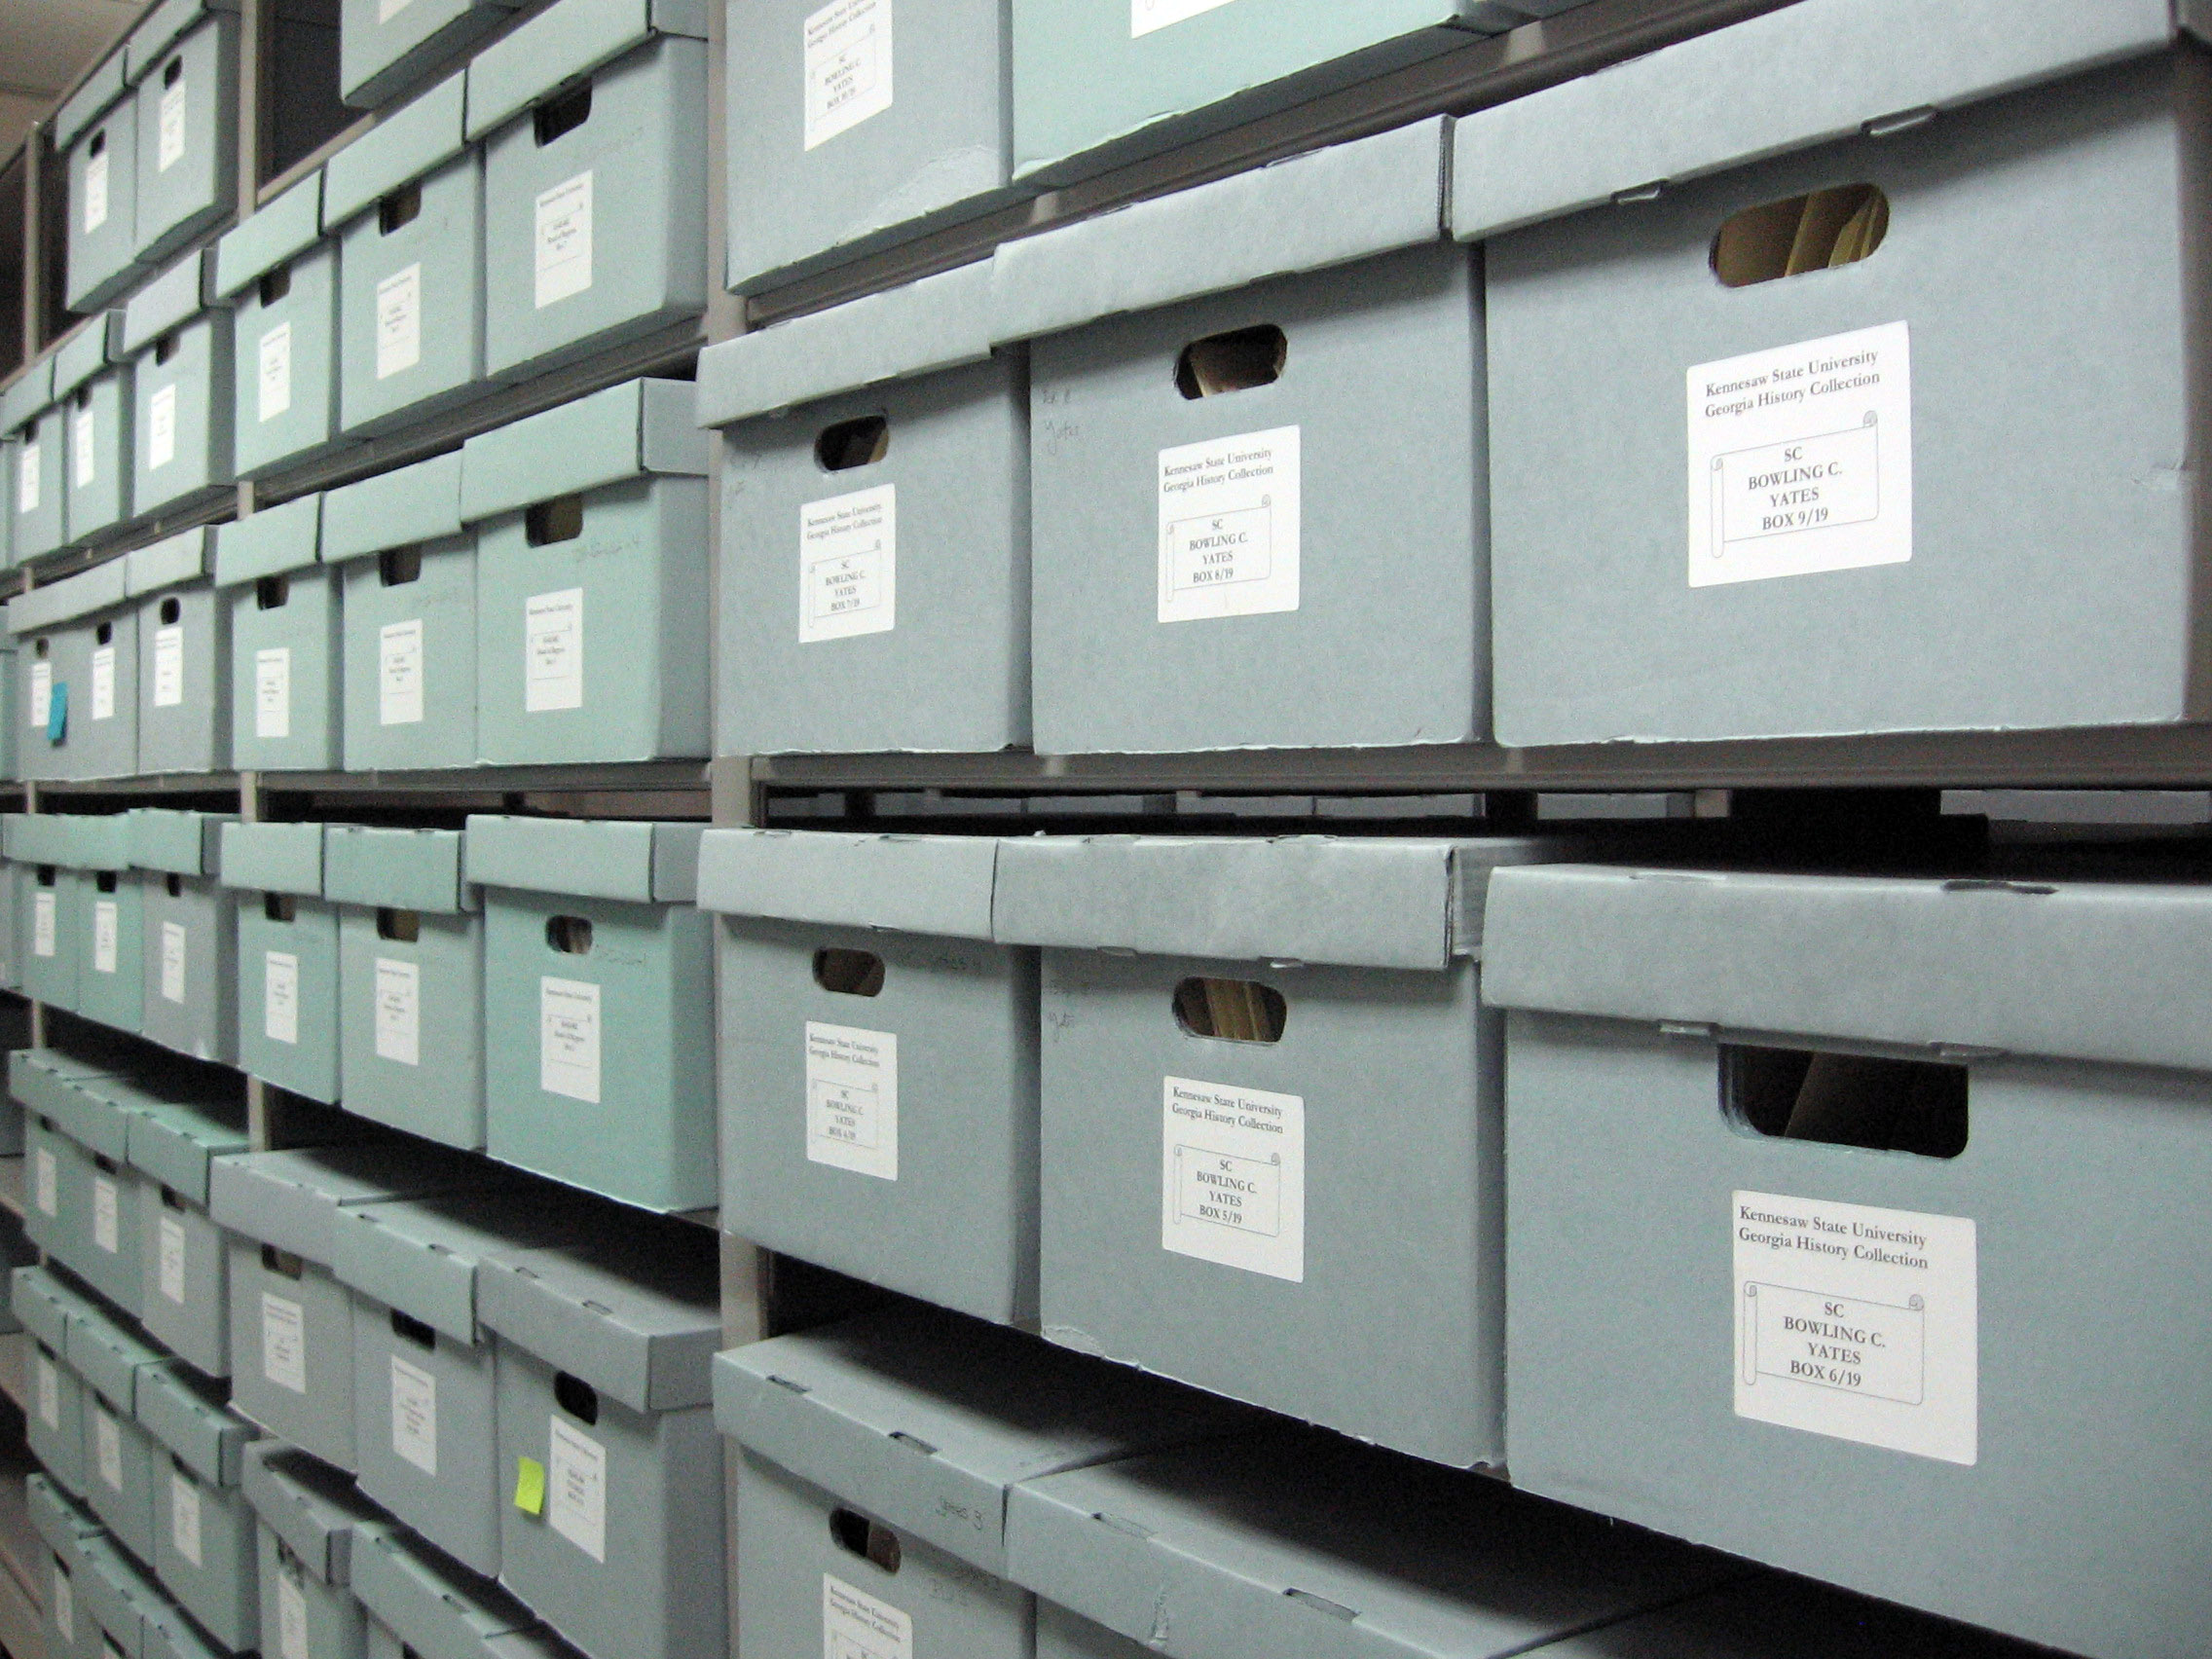
\includegraphics[width=1.5\paperwidth]{archive}}
            \begin{frame}{Abbiamo gli archivi pieni}
                \colorbox{yellow!20}{
                    \begin{minipage}[t]{\paperwidth}
                        Abbiamo realizzato:
                        \begin{itemize}
                            \item documentazione cartacea: schede US
                            \item documentazione grafica: file CAD e tavole stampate
                        \end{itemize}
                    \end{minipage}
                }
            \end{frame}
        }
        % https://secure.flickr.com/photos/dolescum/3568499590/

        \begin{frame}{In altri tempi\ldots}
            La produzione di dati archeologici non era direttamente collegata alla fruizione. I dati finivano in archivio e la fruizione si basava soprattutto sulla rielaborazione di contenuti pubblicati (articoli, cataloghi, ecc.).
        \end{frame}

        \begin{frame}{Oggi}
            Nelle realtà più moderne, esiste continuità tra i dati prodotti durante lo studio del sito e fruizione.\\
            Tra i dati più comunemente utilizzati in ambito turistico:
            \begin{itemize}
                \item cartografia, ortofoto, sistemi di posizionamento in generale
                \item fotografie
                \item riproduzioni 3D di reperti
            \end{itemize}
        \end{frame}

        {
            \usebackgroundtemplate{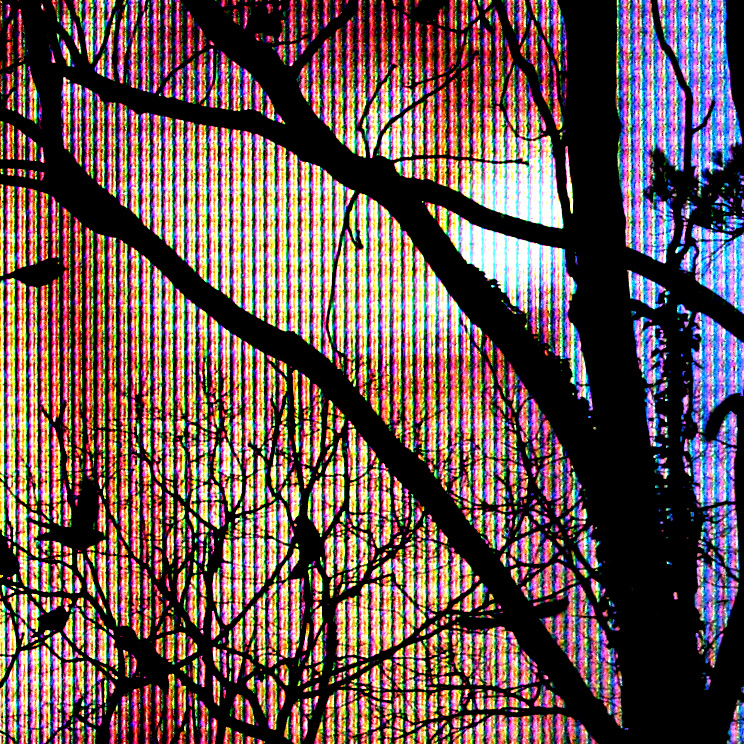
\includegraphics[width=1.5\paperwidth]{multimedia}}
            \begin{frame}{Il nuovo archeologo}
                \colorbox{yellow!20}{
                    \begin{minipage}[t]{\paperwidth}
                        Di conseguenza, il profilo dell'archeologo\\contemporaneo cambia; impara a gestire:
                        \begin{itemize}
                            \item software GIS
                            \item analisi statistica
                            \item database dati (testuali e geografici)
                            \item database multimediali (vedi \emph{DAM})
                            \item borderline: relizzazione prodotti su web / multimediali
                        \end{itemize}
                    \end{minipage}
                }
            \end{frame}
        }
        % https://secure.flickr.com/photos/southernpixel/2215967174

    \section{Digitalizzazione}

        \begin{frame}{Ricominciamo}
            Il prossimo passo?
            \begin{enumerate}
                \item digitalizzare le schede di US
                \item digitalizzare i dati (transizione verso dati geografici)
                \item fusione delle due sorgenti dati
            \end{enumerate}
        \end{frame}

        \subsection{Digitalizzazione delle schede}

            \begin{frame}{Digitalizzare le schede di US}
                Alcuni punti da tenere a mente:
                \begin{itemize}
                    \item tabella del foglio di calcolo come scheda US: ottimo punto di partenza
                    \item formato più semplice per cominciare: CSV
                    \item importanza di UID e dizionari unificati
                \end{itemize}
                \begin{center}
                    \begin{tikzpicture}[node distance = 2cm, auto]
                        \node [roundbox] (carta) {scheda};\pause
                        \node [roundbox, right of=carta] (xls) {\textsc{.xls}};
                        \draw [->] (carta) to (xls);\pause
                        \node [roundbox, right of=xls] (csv) {\textsc{.csv}};
                        \draw [->] (xls) to (csv);\pause
                    \end{tikzpicture}
                \end{center}
            \end{frame}

        \subsection{Cos'è un dato geografico}

            {
                \usebackgroundtemplate{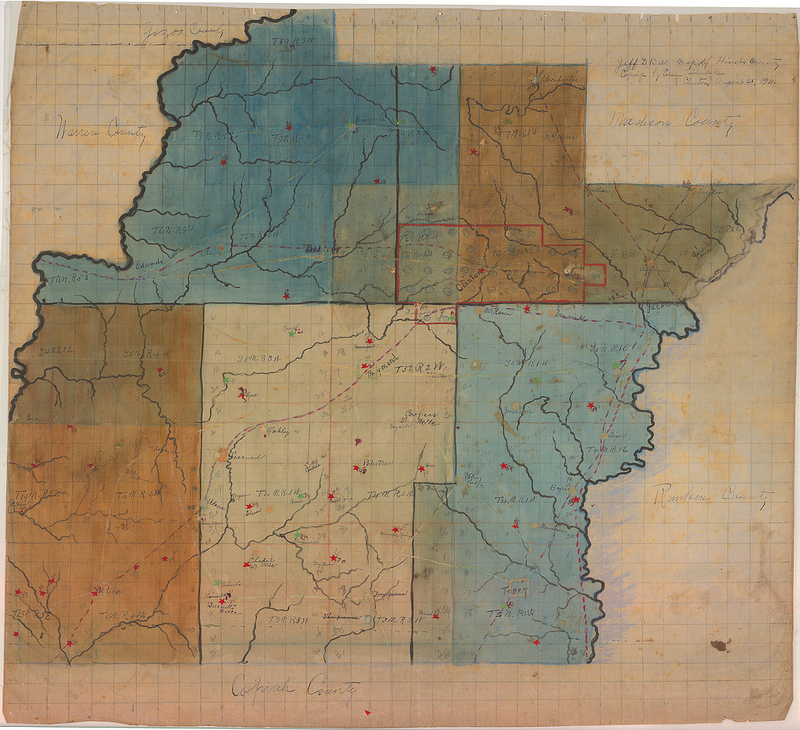
\includegraphics[width=1.5\paperwidth]{map}}
                \begin{frame}{Digitalizzazione dati CAD}
                    \colorbox{yellow!20}{
                        \begin{minipage}[t]{\paperwidth}
                            \begin{itemize}
                                \item cos'è un dato geografico
                                \item formato di transizione: \textsc{dxf}
                                \item georeferenziazione e proiezione: perché sono importanti
                                \item formato di destinazione: \textsc{shapefile} (\textsc{.shp})
                            \end{itemize}
                        \end{minipage}
                    }
                \end{frame}
            }
            % http://www.flickr.com/photos/77015680@N05/7352301434

            \begin{frame}{Il concetto di dato geografico}
                \begin{definition}
                    Insieme di dati (geometrie) a cui sono associate delle coordinate geografiche che permettono la loro individuazione sul globo terrestre (tipologie: \emph{punto}, \emph{linea}, \emph{poligono}).
                \end{definition}\pause
                \vfill
                \begin{tikzpicture}[blue, thick, text=blue!60, scale=0.7]
                    \draw [rounded corners, blue] (-0.,6.5) rectangle (3,11);
                    \node at (1.5, 10.5){\mysize{shapefile}};
                    \draw [thin] (0,10) -- (3,10);
                    \node (us-1) at (1.5,9.5){\mysize{US 1}};
                    \node at (1.5,9){\mysize{US 2}};
                    \node at (1.5,8.5){\mysize{US 3}};
                    \node (us-4) at (1.5,8){\mysize{US 4}};\pause
                    \node [block] (geom-us-1) at (7,9.5) {$P_1$(lat, lon)};
                    \draw [thin] (us-1) -- (geom-us-1);\pause
                    \node [block] (geom-us-4) at (12,8) {$P_1$(lat, lon)\linebreak$P_2$(lat, lon)\linebreak$P_3$(lat, lon)\linebreak$P_4$(lat, lon)};
                    \draw [thin] (us-4) -- (geom-us-4);
                \end{tikzpicture}
            \end{frame}

            \subsection{Da \textsc{.dwg} a \textsc{.shp}}

                \begin{frame}{Schema delle esportazioni}
                    \begin{center}
                        \begin{tikzpicture}[node distance = 2cm, auto]
                            \node [roundbox] (dwg) {\textsc{.dwg}};\pause
                            \node [transitionbox, right of=dwg] (pulizia) {pulizia};
                            \draw [->] (dwg) to (pulizia);\pause
                            \node [roundbox, right of=pulizia] (dxf) {\textsc{.dxf}};
                            \draw [->] (pulizia) to (dxf);\pause
                            \node [transitionbox, right of=dxf] (georef) {{\tiny{georeferenziazione}}};
                            \draw [->] (dxf) to (georef);\pause
                            \node [roundbox, right of=georef] (shp) {\textsc{.shp}};
                            \draw [->] (georef) to (shp);\pause
                            \node [below of=pulizia] (autocad) {\emph{AutoCAD}};
                            \node [below of=georef] (qgis) {\emph{QuantumGIS}};
                        \end{tikzpicture}
                    \end{center}
                \end{frame}

            \subsection{Perchè è importante georeferenziare}

                \begin{frame}{Perché georeferenziare}
                    \begin{itemize}
                        \item la Terra non è piatta
                        \item tutti i geo-database ``masticano'' esclusivamente dati georeferenziati
                        \item la cartografia in \textsc{.shp} è più ordinata di quella in \textsc{.dwg}
                        \item i dati georeferenziati possono integrare collezioni di dati geografici esistenti (carta archeologica)
                    \end{itemize}
                    \vfill\pause
                    Occorre comunque fare attenzione: in alcuni casi (rendering e ricostruzioni 3D) è più pratico
                    lavorare su \textsc{.dwg} piuttosto che su altri formati.
                \end{frame}

            \subsection{Fondere i dati}

                \begin{frame}{Fondere schede e geografia}
                    \begin{description}
                        \item[perchè] interrogazioni congiunte, maggiori informazioni rispetto alla somma dei singoli dati
                        \item[dove] in un database (ideale PostGIS --- gratis!)
                        \item[cos'è] una grande tabella, con funzioni avanzate che danno risposte veloci a domande complesse
                        \item[con~cosa] QGIS (gratis!)
                    \end{description}
                \end{frame}

                \begin{frame}{Dai dati al database}
                    \begin{tikzpicture}[node distance = 2cm, auto]
                        \node [roundbox] (csv) {\textsc{.csv}};\pause
                        \node [right of=csv] (plus) {+};
                        \node [roundbox, right of=plus] (shp) {\textsc{.shp}};\pause
                        \draw [rounded corners, blue] (-1,-0.5) rectangle (5,0.5);\pause
                        \node [roundbox, below of=shp, distance = 1cm] (postgis) {geo-database};\pause
                        \path [->, font=\scriptsize] (shp) edge node {QGIS} (postgis);
                    \end{tikzpicture}
                \end{frame}

                \begin{frame}{Unire due tabelle}
                    \begin{block}{Come è possibile unire dati di natura differente?}
                        Perché (in fondo) \textsc{.shp} e \textsc{.csv} sono entrambi \emph{tabelle}, ed hanno in comune un \emph{indice}.
                    \end{block}\pause
                    \begin{center}
                        \begin{tikzpicture}[blue, thick, text=blue!60, scale=0.7]
                            \draw [rounded corners, blue] (-0.,7.5) rectangle (4,11);
                            \node at (1.5, 10.5){\mysize{shapefile}};
                            \draw [thin] (0,10) -- (4,10);
                            \node at (1.5,9.5){\mysize{US 1}};
                            \node (shp1) at (3,9.5){\mysize{1}};
                            \node at (1.5,9){\mysize{US 2}};
                            \node (shp2) at (3,9){\mysize{2}};
                            \node at (1.5,8.5){\mysize{US 3}};
                            \node (shp3) at (3,8.5){\mysize{3}};
                            \node at (1.5,8){\mysize{US 4}};
                            \node (shp4) at (3,8){\mysize{4}};\pause
                            \draw [rounded corners, blue] (7,7.5) rectangle (11,11);
                            \node at (8.5, 10.5){\mysize{csv}};
                            \draw [thin] (7,10) -- (11,10);
                            \node at (9.5,9.5){\mysize{scheda 1}};
                            \node (csv1) at (8,9.5){\mysize{1}};
                            \node at (9.5,9){\mysize{scheda 2}};
                            \node (csv2) at (8,9){\mysize{2}};
                            \node at (9.5,8.5){\mysize{scheda 3}};
                            \node (csv3) at (8,8.5){\mysize{3}};
                            \node at (9.5,8){\mysize{scheda 4}};
                            \node (csv4) at (8,8){\mysize{4}};\pause
                            \draw (shp1) -- (csv1);
                            \draw (shp2) -- (csv2);
                            \draw (shp3) -- (csv3);
                            \draw (shp4) -- (csv4);
                        \end{tikzpicture}
                    \end{center}
                \end{frame}

\part{Ora siamo ancora più ordinati. Che si fa?}
	\frame{\partpage}

    \section{Ordinare vs Gestire}

        \begin{frame}{Ordinare è diverso da gestire}
            Il nostro sistema dovrà permetterci di:
            \begin{itemize}
                \item aggiungere ed eliminare dati rapidamente
                \item ottenere informazioni rapidamente
                \item essere utilizzabile dagli archeologi: serve un'interfaccia
            \end{itemize}
        \end{frame}

        \begin{frame}{Alcune interrogazioni utili}
            Il valore dei dati ordinati in un database è superiore alla sola somma dei valori inseriti,
            grazie alle informazioni che si possono estrarre dalle interrogazioni (\emph{query}):
            \begin{itemize}
                \item dalle US datate al X secolo, estrarre i soli frammenti in vetro bugnati
                \item estrarre la datazione delle US nelle quali sono stati rinvenuti frammenti di sigillata con la stessa composizione chimica
                \item per ogni fase, estrarre la quantità relativa di ceramiche, vetro e metalli
            \end{itemize}\pause
            \begin{block}{Per approfondire}
                \emph{Archeologia quantitativa}
            \end{block}
        \end{frame}

    \section{L'importanza delle interfacce}

        \begin{frame}{Interfaccia alle schede US: ARK}
            \begin{itemize}
                \item utilizzabile via internet: cos'è un server?
                \item utilizzabile contemporaneamente da vari utenti
                \item permette importazione di grosse quantità di dati
                \item albero dei dati estendibile all'infinito (a differenza di scheda US e\ldots Microsoft Access)
            \end{itemize}\pause
            \begin{block}{Live}
                \url{http://ark.sipontomedievale.it}
            \end{block}
        \end{frame}

        \begin{frame}{I server dati archeologici}
            \begin{figure}
                \centering
                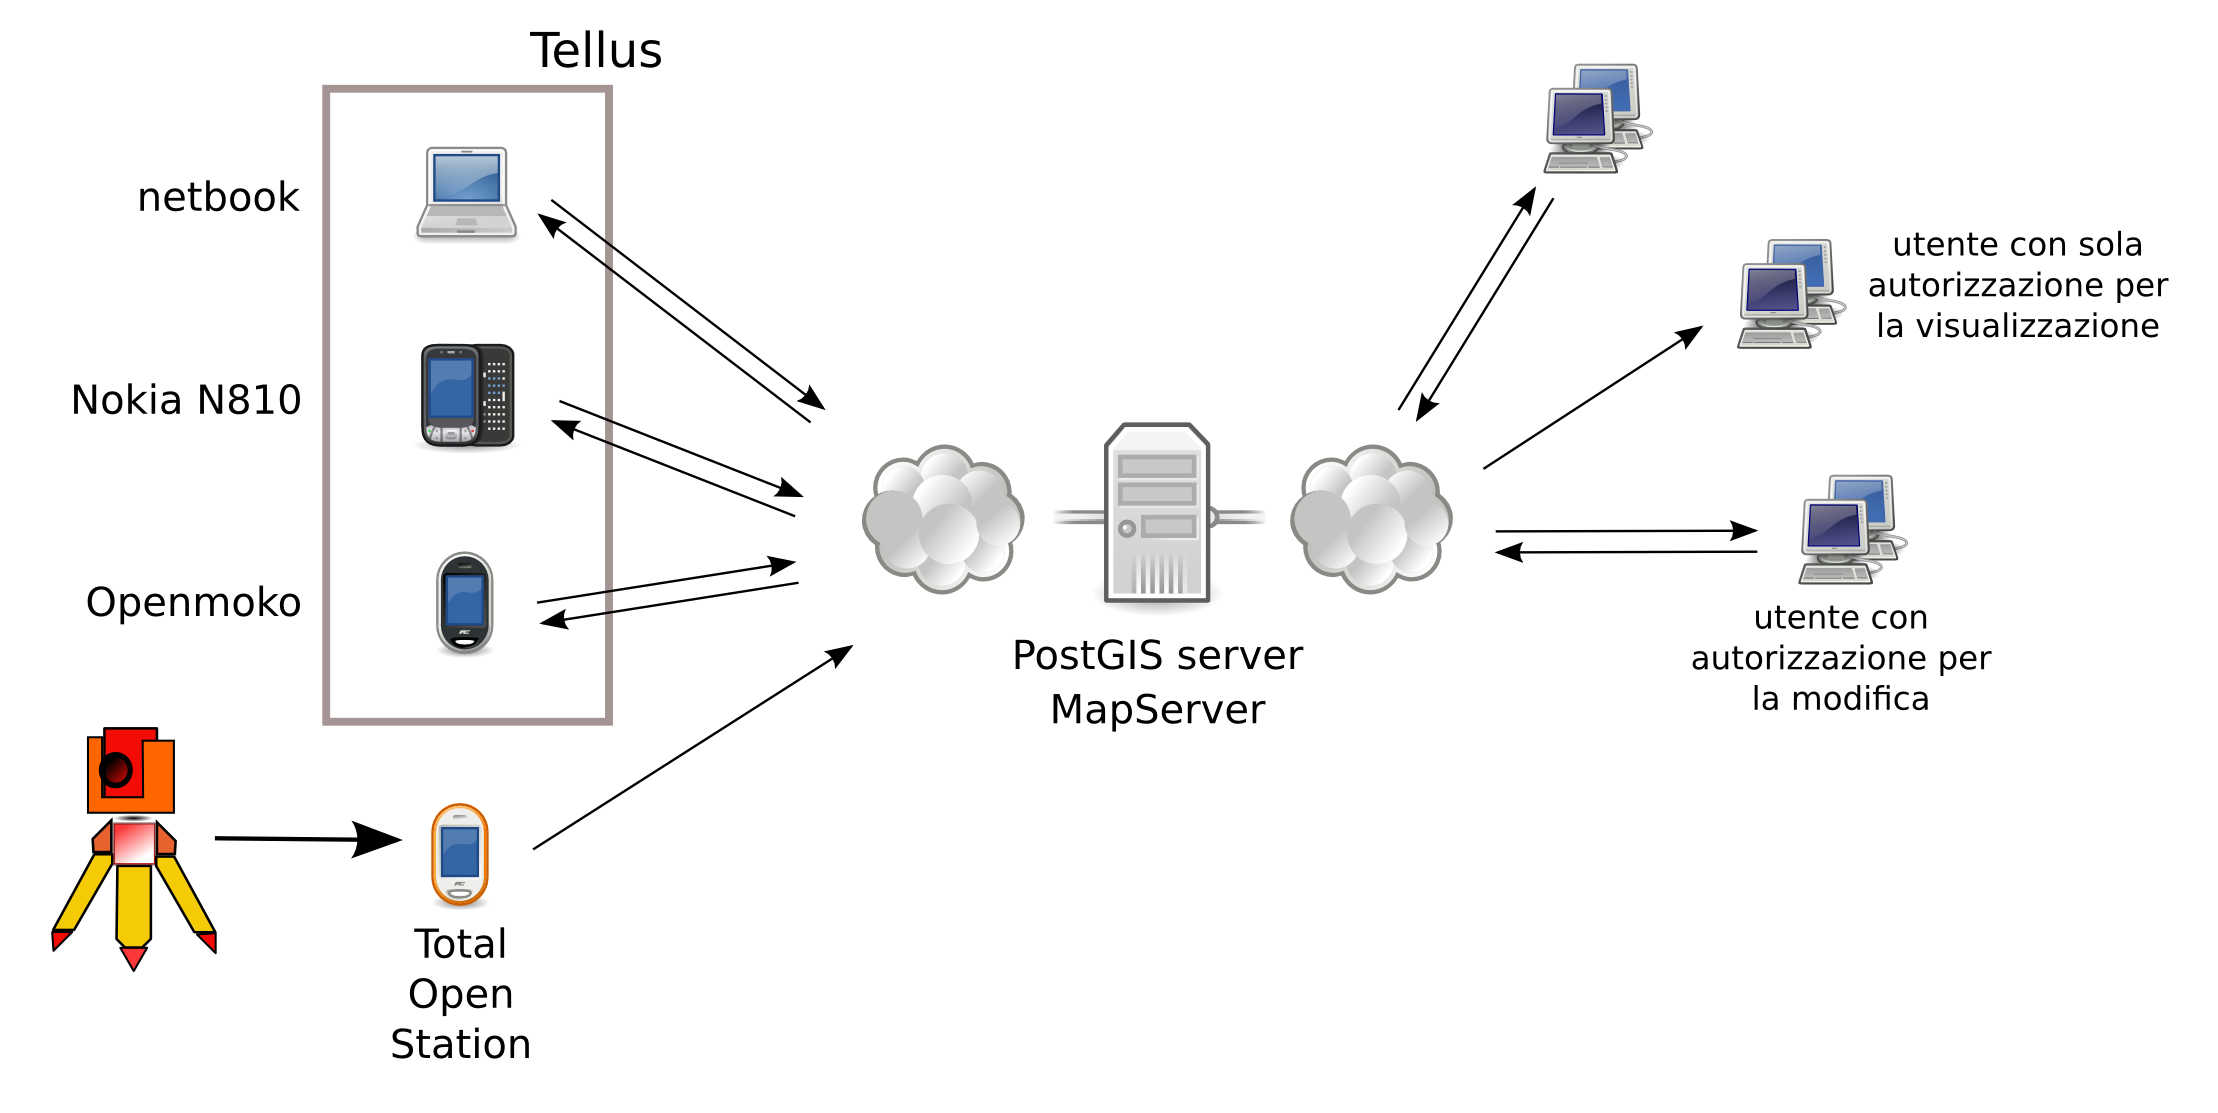
\includegraphics[width=1\linewidth]{schematellus}
                \caption[Un sistema client/server per la gestione dei dati archeologici]{Un sistema client/server per la gestione dei dati archeologici}
                \label{fig:tellus}
            \end{figure}
        \end{frame}

        \begin{frame}{Interfaccia per i dati geografici}
            \begin{columns}[c]
                \column{.5\textwidth} 
                    \begin{center}
                        \emph{Desktop}
                            \begin{itemize}
                                \item software da installare su PC
                                \item permette di eseguire tutte le operazioni sui dati geografici
                                \item può gestire dati sul PC o su server (PostGIS)
                                \item ideale per la gestione, meno per la fruizione
                            \end{itemize}
                    \end{center}
                    \column{.5\textwidth}
                    \begin{center}
                        \emph{Web}
                        \begin{itemize}
                            \item anche detti \emph{webGIS}; non si installano
                            \item ottimi visualizzatori, in alcune occasioni permettono di gestire i dati
                            \item visualizzano quasi solo dati su server
                            \item ideale per la fruizione: integrazione con altri contenuti web
                        \end{itemize}
                    \end{center}
            \end{columns}
        \end{frame}

\part{Siamo ordinati e sappiamo gestire. Ci fermiamo?}
	\frame{\partpage}

    \begin{frame}{No!}
        \centering
        \Huge
        Adesso, finalmente, realizziamo prodotti professionali
    \end{frame}

    \section{Dietro le quinte del web}

        \begin{frame}{Costruire prodotti per il pubblico}
            Concetti generali
            \begin{itemize}
                \item cos'è un servizio web
                \item web e desktop mobile
                \item gli standard web: \textsc{HTML}, \textsc{CSS}, \textsc{geojson}
            \end{itemize}
        \end{frame}

    \section{Esempi pratici}

        \begin{frame}{In soldoni: Siponto Aperta}
            \centering
            \url{http://www.sipontoaperta.it}
            \vfill
			\begin{figure}[]
				\begin{center}
					
\includegraphics[width=0.2\linewidth]{regione}\hfill
					
\includegraphics[width=0.3\linewidth]{pa}
				\end{center}
				\label{fig:regione}
			\end{figure}
            \vfill
            \begin{description}
                \item[tour~immersivo] GIS + HTML5 + foto
                \item[webGIS] MySQL + GIS + HTML5 + 3D
            \end{description}
        \end{frame}

        \begin{frame}{Comunicare lo scavo}
            \begin{columns}[c]
                \column{.5\textwidth}
                    \begin{itemize}
                        \item webGIS, 3D su web
                        \item blog, diario di scavo
                        \item social network
                    \end{itemize}
                \column{.5\textwidth}
                \begin{figure}
                    \centering
                    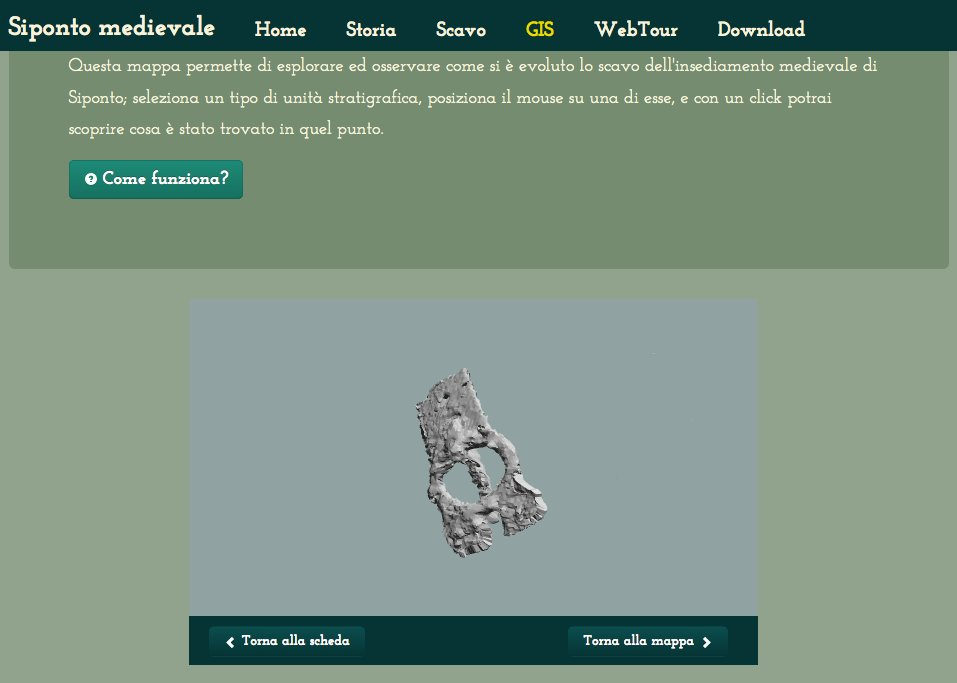
\includegraphics[width=1\textwidth]{screen_3d}
                    \caption[Riproduzione 3D di reperto sul web]{Riproduzione 3D di reperto sul web}
                    \label{fig:3dweb}
                \end{figure}
            \end{columns}
        \end{frame}

    \section{Note}

        \begin{frame}{In un mondo ideale, dovremmo evitare\ldots}
            \begin{description}
                \item[database~locali] su pc desktop, non raggiungibili via internet; eliminano la collaborazione a distanza e la possibilità di sviluppare prodotti web
                \item[software~proprietario] in ambito database/geografico non presenta nessun vantaggio concreto rispetto al software libero
                \item[siti~web~statici] le nuove tecnologie web sono dinamiche, usano \emph{framework}; i prodotti web sono disponibili simultaneamente per desktop, tablet, smartphone
            \end{description}
        \end{frame}

        \begin{frame}{Materiali utili}
            \begin{description}
                \item[Spazio e Misura]manuale di statistica geografica, libera distribuzione in PDF\\\url{http://www.archeogr.unisi.it/testi}
                \item[GRASS per archeologi]introduzione all'utilizzo di GRASS GIS in Archeologia, libera distribuzione in PDF\\\url{http://github.com/fradeve/grass-arch}
                \item[Archeologia e Calcolatori]dal 1990 si occupa di informatica applicata all'archeologia; PDF in libera distribuzione\\\url{http://www.progettocaere.rm.cnr.it/databasegestione/google_year_list.htm}
            \end{description}
        \end{frame}

\end{document}
